%% LyX 1.3 created this file.  For more info, see http://www.lyx.org/.
%% Do not edit unless you really know what you are doing.
\documentclass[english]{article}
\usepackage[latin1]{inputenc}
\usepackage{geometry}
\geometry{verbose,a4paper}
\usepackage{subfigure}
\usepackage{amsmath}
\usepackage{graphicx}
\usepackage{amssymb}
\IfFileExists{url.sty}{\usepackage{url}}
                      {\newcommand{\url}{\texttt}}
\usepackage[authoryear]{natbib}

\makeatletter
\AtBeginDocument{
  \renewcommand{\labelitemi}{\color{gold}\ding{122}\color{foreground}}
  \renewcommand{\labelitemii}{\color{gold}\ding{229}\color{foreground}}
  \renewcommand{\labelitemiv}{\ding{229}}
}

\usepackage{babel}
\makeatother
\begin{document}

\title{Gaussian Process Models for Single Input Motif Networks}


\author{Guido Sanguinetti, Neil D. Lawrence and Magnus Rattray}

\maketitle
\begin{abstract}
In this paper we show how protein concentration can be inferred from
gene expression data using Gaussian process models. We consider the
situation where serveral genes are regulated by a single parent. We
follow recent work by \cite{Barenco:ranked06} in assuming that the
relationship between the genes and the governing protein can be modelled
by a simple linear differential equations. We compare our results
to those of \citeauthor{Barenco:ranked06} and suggest extensions
to the model for which the differential equation need not be linear.
\end{abstract}

\section{Introduction}

Advances in microarray technology over the last ten years have meant
that large scale direct measurements of gene expression is now possible.
Unfortunately, the same can not be said about the measurement of protein
expression. Transcription factors are proteins that have a key influence
on the operation of genetic networks. While they are often governed
by at most one gene, that gene is typically a poor proxy for the transcription
factor's protein. There is, therefore, a great deal of interest in
inferring transcription factor's protein concentrations indirectly
through known targets of the transcription factor. To this end ChIpCHip
DaTa (reference) can be combined with microarray data to give information
about the transcription factors' targets on a genome wide scale, see
for example \citet{Liao:nca03,Boulesteix:predicting05,Sanguinetti:chipdyno06}.
However, such genome-wide models necessarily make strong simplifying
assumptions concerning the interactions. In this paper we follow the
alternative approach of focussing on a sub-network, in this case focussing
only on one transcription factor, but using a more detailed model
of the interactions than can practically be applied in genome-wide
studies. 


\section{Sub-Networks}

We follow \citet{Barenco:ranked06} in considering a linear differential
equation that relates a given gene's expression to the concentration
of its parent,\begin{equation}
\frac{dx_{j}\left(t\right)}{dt}=B_{j}+S_{j}f\left(t\right)-D_{j}x_{j}\left(t\right),\label{eq:diffEqn}\end{equation}
where $x_{j}\left(t\right)$ is the expression level of gene $j$
at time $t$, $f\left(t\right)$ is the concentration of the transcription
factor protein at time $t$, $B_{j}$ is the basal transcription rate
of gene $j$, $S_{j}$ is the sensitivity of gene $j$ to the transcription
factor and $D_{j}$ is the decay rate of the genes mRNA. This differential
equation is also a simplification of the true relationship but \citet{Barenco:ranked06}
found that it achieved good results in modelling relationships between
the transcription factor (TF) p53 (a key TF in tumor suppression)
and its targets.

\citeauthor{Barenco:ranked06} selected five targets of p53 and modelled
their expression levels using polynomial curve fitting. They then
used Markov chain Monte Carlo (MCMC) to estimate the protein concentration
at each time point as well as the basal transcription rate, the sensitivity
and the decay for each gene. Their approach has two significant defects.
Firstly, there model includes no concept of temporal continuity that
would allow the protein concentration level to be interpolated between
time points. Secondly, they needed to make use of numerical solutions
to solve their differential equation and had to perform up to 10 million
steps of MCMC in the parameter estimation stage. 

In this paper we show how the entire model can be resolved using a
Gaussian process prior on the protein concentration. We achieve similar
results to \citet{Barenco:ranked06} without having to resort to numerical
solutions of the equation or Markov chain Monte Carlo. We then show
how our methodology can be extended to non-linear differential equations
using MAP approximations to the process posterior.


\section{Gaussian Process Model}

The equation given in (\ref{eq:diffEqn}) can be solved to recover\[
x_{j}\left(t\right)=\frac{B_{j}}{D_{j}}+k_{j}\exp\left(-D_{j}t\right)+S_{j}\exp\left(-D_{j}t\right)\int_{0}^{t}f\left(u\right)\exp\left(-D_{j}u\right)du\]
where $k_{j}$ arises from the initial conditions, and can be assumed
to be zero if the system has reached steady state. Importantly this
equation involves on linear operations on the function $f\left(t\right)$.
This means that if we place a Gaussian process prior over $f\left(t\right)$
this directly implies a Gaussian process prior over $x_{j}\left(t\right)$.
If the covariance function associated with $f\left(t\right)$ is given
by $k_{ff}\left(t,t^{\prime}\right)$ then the covariance function
associated with $x_{j}\left(t\right)$ is given by\[
k_{x_{j}x_{j}}\left(t,t^{\prime}\right)=S_{j}^{2}\exp\left(-D_{j}\left(t+t^{\prime}\right)\right)\int_{0}^{t}\exp\left(-D_{j}u\right)\int_{0}^{t^{\prime}}\exp\left(-D_{j}u^{\prime}\right)k_{ff}\left(u,u^{\prime}\right)du^{\prime}du,\]
however to predict $f\left(t\right)$ given instantiations of$\left\{ x_{j}\left(t\right)\right\} _{j=1}^{m}$
we also need the `cross-covariance' terms between $x_{i}\left(t\right)$
and $x_{j}\left(t^{\prime}\right)$, $k_{x_{i}x_{j}}\left(t,t^{\prime}\right)$
and between $x_{j}\left(t\right)$ and $f\left(t^{\prime}\right)$,
$k_{x_{j}f}\left(t,t^{\prime}\right)$. These can be computed through\[
k_{x_{i}x_{j}}\left(t,t^{\prime}\right)=S_{j}S_{i}\exp\left(-D_{i}t-D_{j}t^{\prime}\right)\int_{0}^{t}\exp\left(-D_{i}u\right)\int_{0}^{t^{\prime}}\exp\left(-D_{j}u^{\prime}\right)k_{ff}\left(u,u^{\prime}\right)du^{\prime}du\]
and\[
k_{x_{j}f}\left(t,t^{\prime}\right)=S_{j}\exp\left(-D_{j}t\right)\int_{0}^{t}\exp\left(-D_{j}u\right)k_{ff}\left(u,t^{\prime}\right)du\]
respectively. Furthermore, if the process prior over $f\left(t\right)$
is taken to be a squared exponential kernel, \[
k_{ff}\left(t,t^{\prime}\right)=\exp\left(-\frac{\left(t-t^{\prime}\right)^{2}}{\sigma^{2}}\right),\]
where $\sigma$ controls the width of the basis functions%
\footnote{The scale of the process is ignored to avoid a parameterisation ambiguity
with the sensitivities.%
}, all the integrals can be computed analytically. We can therefore
compute a likelihood which relates instantiations from all the observed
genes, $\left\{ x_{j}\left(t\right)\right\} _{j=1}^{m}$, through
dependencies on the parameters $\left\{ B_{j},S_{j},D_{j}\right\} _{j=1}^{m}$.
The effect of $f\left(t\right)$ has been marginalised. This allows
us to avoid sampling over $f\left(t\right)$ in the manner of \citet{Barenco:ranked06,Rogers:model06},
both of which necessarily restrict samples of $f\left(t\right)$ to
the instantiations of $f\left(t\right)$ that are associated with
time points were measurements are taken. 


\section{Experiments}

To demonstrate the efficacy of our approach, we followed \citet{Barenco:ranked06}
in analysing five targets of p53: \emph{DDB2}, \emph{p21} \emph{SESN1/hPA26},
\emph{BIK} and \emph{TNFRSF10b}. Results, including comparisions with
results of \citeauthor{Barenco:ranked06} are given in Figure~\ref{cap:barencoComparisonBar}~and~.

%
\begin{figure}[h]
\begin{center}\subfigure[]{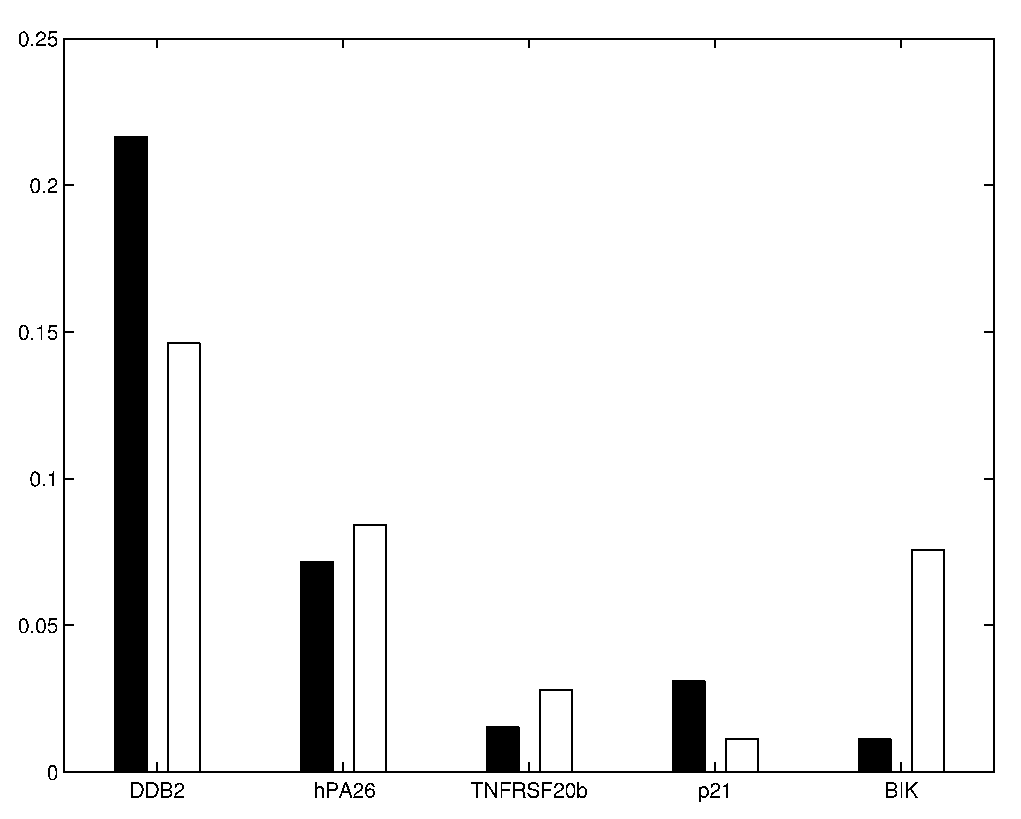
\includegraphics[%
  width=0.30\textwidth]{../diagrams/demBarenco1_basal.eps}}\hfill{}\subfigure[]{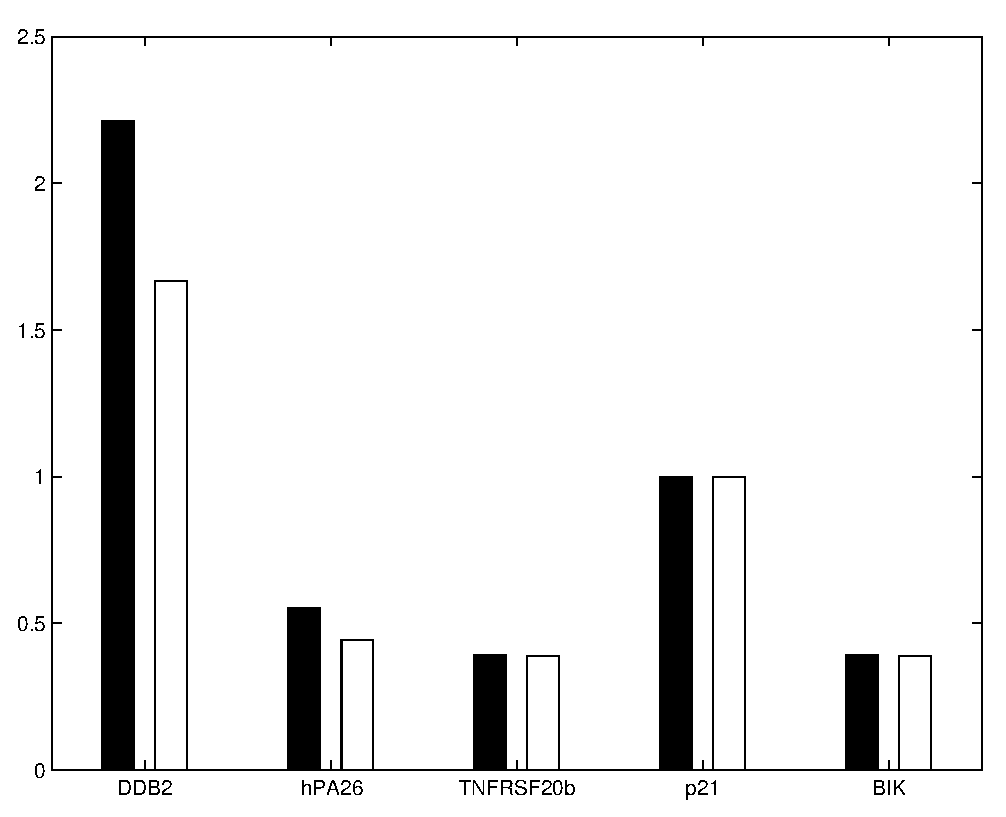
\includegraphics[%
  width=0.30\textwidth]{../diagrams/demBarenco1_sensitivity.eps}}\hfill{}\subfigure[]{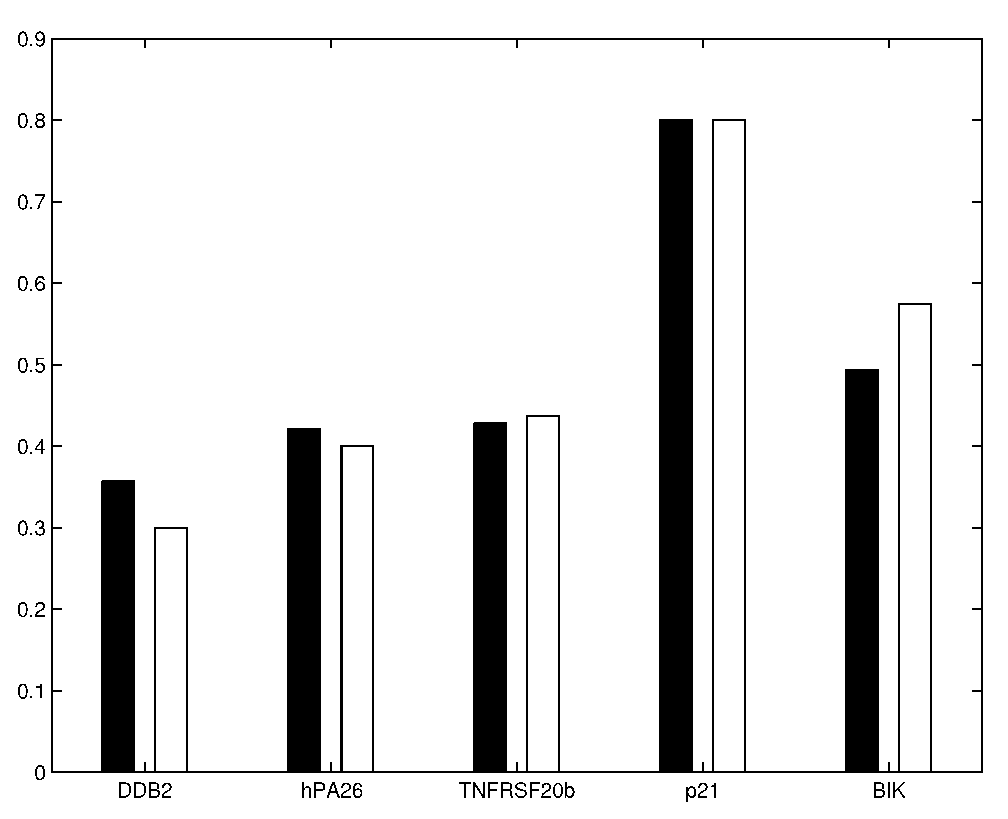
\includegraphics[%
  width=0.30\textwidth]{../diagrams/demBarenco1_decay.eps}}\end{center}


\caption{Results of inference on p53 data of \citeauthor{Barenco:ranked06}.
The bar charts show (a) Basal transcription rates from our model and
that of \citeauthor{Barenco:ranked06}. White shows results from our
model, black is \citeauthor{Barenco:ranked06}. (b) Similar for sensitivities.
(c) Similar for decay rates.\label{cap:barencoComparisonBar}.}
\end{figure}


As can be seen from the bar plots, our results in terms of degradations,
sensitivities and basal transcription rates are strikingly similar
to those of \citeauthor{Barenco:ranked06}. However, ours were obtained
in approximately 13 minutes in MATLAB on an AMD Athlon 1.79 GHz machine
using approximately 600 iterations conjugate gradient optimisation
(see \url{http://www.dcs.shef.ac.uk/~neil/gpsim} for the code used).
Timings aren't given by \citeauthor{Barenco:ranked06}; they used
10 million iterations of MCMC to obtain their results.

%
\begin{figure}[h]
\begin{center}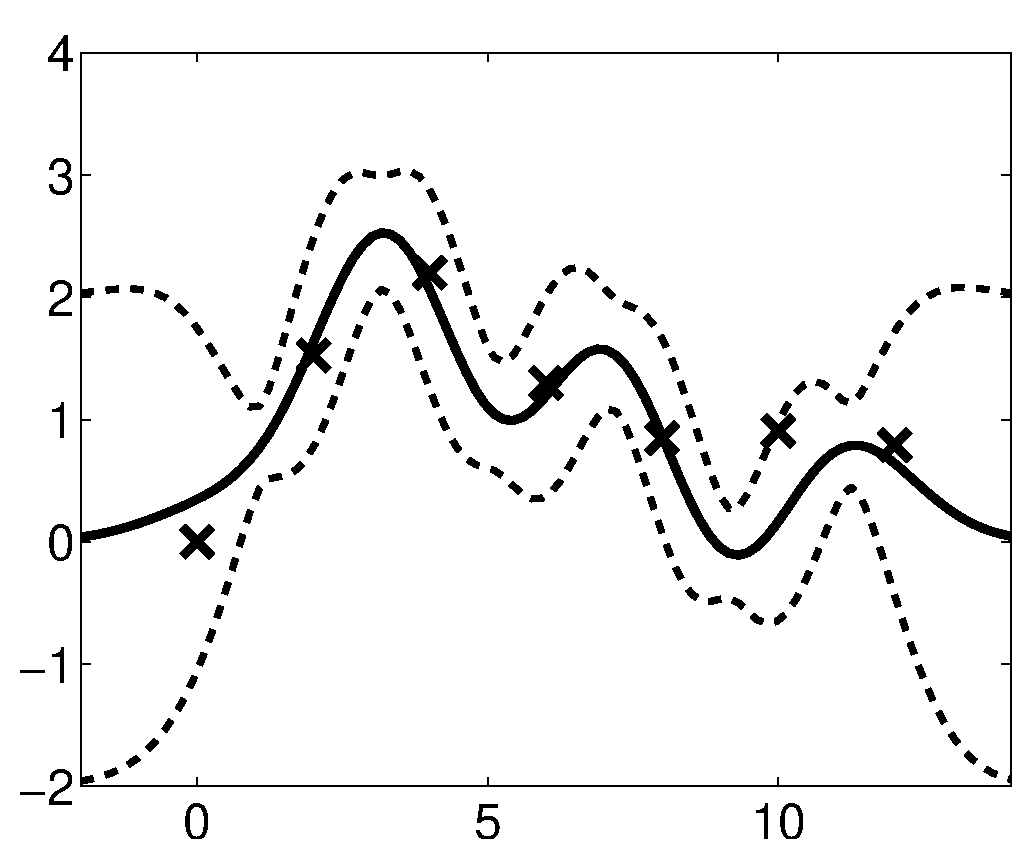
\includegraphics[%
  scale=0.4]{../diagrams/demBarenco1_profile1.eps}\end{center}


\caption{Predicted concentration for p53. Solid line is mean prediction, dashed
lines are at two standard deviations. The prediction of \citeauthor{Barenco:ranked06}
was pointwise and is shown as crosses.}
\end{figure}



\section{Non-linear Equations}

We know how to do them too ... aren't we clever!


\subsection*{Acknowledgements}

Martino was quite helpful ... should really say something to thank
him.

\bibliographystyle{plainnat}
\bibliography{lawrence,other,zbooks}

\end{document}
